\section{Schlussfolgerungen
\label{section:conclusions}}
Anhand der in den Abschnitten~\ref{section:iosmeasurements} 
und~\ref{section:androidmeasurements} genannten Resultate lassen sich nun 
mehrere Verfahren für eine Unterscheidung von Mobilgeräten herleiten.

Hier gilt zu erwähnen, dass die durchgeführten Messungen in dieser Bachelorarbeit
statistisch nicht signifikant sind, da lediglich für das Samsung Galaxy S8 
Tests auf mehr als zwei unterschiedlichen Geräten durchgeführt wurden.
Dies Bedeutet, dass eine Beobachtung, die spezifisch auf einem Gerät gemacht 
wurde, (z.B. Die hauptsächliche Verwendung der MAC-\\Adresse "02:00:00:00:00:00" 
auf dem Samsung A51) nicht für alle Geräte dieses Typs gelten müssen.
Verfahren, die ein Mobilgerät aufgrund der spezifischen Eigenschaften dieses 
Geräts erkennen, können in der Praxis daran scheitern, dass das zu Messende
Gerät sich anders verhält als andere Geräte der selben Bauart.

Trotzdem wurden einige Beobachtungen gemacht, die es in Kombination mit den im 
Kapitel~\ref{chapter:analysis} recherchierten Geräteverhalten ermöglichen,
Mobilgeräte unterschiedlicher Bauart voneinander zu unterscheiden.

\clearpage

\subsection{Generelle Ansätze für ein Fingerprinting anhand ausgesendeter Probe-Requests}
Allgemein kann ein Mobilgerät anhand einer oder mehrerer Eigenschaften von 
anderen Geräten eindeutig unterschieden werden. Kann diese Unterscheidung 
mehrmals nacheinander durchgeführt werden, sind diese Eigenschaften oder eine 
Kombination davon für dieses Gerät einzigartig und dienen somit als Fingerabdruck.
Bevor die MAC-Adresse von Mobilgeräten zufallsgeneriert wurde, 
konnte diese Adresse als Fingerprint genutzt werden. 
Die Abbildung~\ref{figure:naivefingerprinting} zeigt dabei konzeptionell, 
wie solch ein Fingerprinting durchgeführt werden könnte.

\begin{figure}[h!]
    \centering
    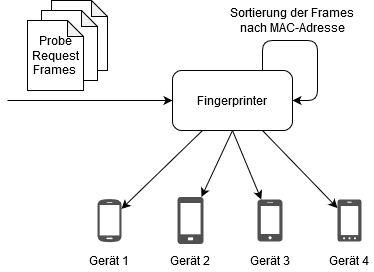
\includegraphics[width=0.8\linewidth]{Experiments/MAC-Fingerprinting.png}
    \caption{Fingerprinting vor iOS 8 / Android 9
    \label{figure:naivefingerprinting}}
\end{figure}

Da die MAC-Adresse in modernen Geräten mit aktuellen Betriebssystemen aber
zufallsgeneriert wird, muss dieses Verfahren angepasst werden.
Ziel ist, Eigenschaften zu finden, um Geräte daran zu unterscheiden.
Dabei gibt es verschiedene Ansätze: Machine Learning-Verfahren versuchen, 
automatisiert aus Millionen von Probe-Requests diese Eigenschaften zu finden 
und Geräte dementsprechend zu unterscheiden.

\clearpage

Ein weiterer Ansatz ist es, automatisiert nach vorgegebenen Filterregeln 
Geräte anhand bekannter Eigenschaften zu sortieren. Diese Filterung kann 
in mehreren Teilschritten vorgenommen werden. Zuerst wird anhand einer 
Eigenschaft sämtliche ankommende oder verfügbare Probe-Requests in diverse 
Gruppen unterteilt. Jede dieser Gruppen kann danach mit weiteren Filtern 
in Untergruppen unterteilt werden. Sind alle Filtervorgänge abge-schlossen,
sollten sämtliche Frames einer Gruppe zu einem eindeutigen Mobilgerät gehören.
Der Ansatz ist in der Abbildung~\ref{figure:sophisticatedfingerprinting} 
konzeptionell dargestellt.

\begin{figure}[h!]
    \centering
    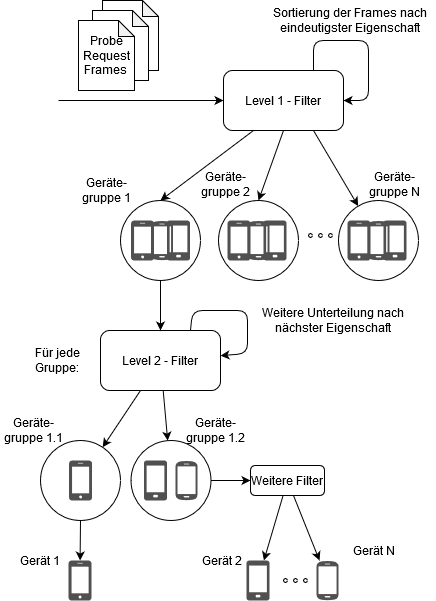
\includegraphics[width=0.8\linewidth]{Experiments/Filter-Fingerprinting.png}
    \caption{Filterbasiertes, hierarchische Geräteunterscheidung
    \label{figure:sophisticatedfingerprinting}}
\end{figure}

\clearpage

Ein Vorteil eines filterbasierten Ansatzes ist, dass neue Erkenntnisse oder 
Änderungen des Geräteverhaltens mit geringem Aufwand implementiert werden können,
indem die Filterregeln dementsprechend angepasst werden. 
Weiterhin muss im Gegensatz zu einem Machine-Learning-Ansatz nicht für jede 
Änderung ein Training des Algorithmus durchgeführt werden (von selbstlernenden
Algorithmen abgesehen). 
Nachteile sind der Aufwand, der benötigt wird, um an die neuen unterscheidbaren
Eigenschaften zu kommen und dass ein Filter-Programm regelmässig 
an die Eigenschaften angepasst werden muss.
Auch hier können selbstlernende Algorithmen eingesetzt werden, um den Aufwand 
zu verringern. 

\clearpage

\subsection{Spezifische Ansätze für die Geräteunterscheidung
\label{subsection:specificapproaches}}
Im Verlaufe der Bachelorarbeit sind mehrere Ansätze entstanden, wie 
eine Unterscheidung von Mobilgeräten durchgeführt werden könnte.
Nachfolgend sind diese Ansätze, deren Vorgehen und die Umsetzbarkeit 
beschrieben.

\subsubsection*{Ansatz 1: Zeitbasierte Auswertung von Frames}
Unabhängig von den Informationen, die in ausgesendeten Probe-Requests enthalten
sind, kann allein aufgrund von zeitlichen Informationen gefiltert werden.
Ein Mobilgerät sendet jeweils einen Burst von Probe-Requests mit der gleichen 
MAC-Adresse aus. Wird innerhalb der Zeit des Bursts ein Frame aufgezeichnet, 
welches eine andere MAC-Adresse hat, wird dieses von einem anderen Gerät 
ausgesendet. 

\paragraph{Vorgehen}
Wenn ankommende Frames in Bursts gruppiert werden, können Frames, die im selben 
Zeitraum aufgezeichnet werden, davon unterschieden werden. 
Allein anhand dieser Information kann eine ungefähre Anzahl von Mobilgeräten 
im Empfangsbereich eines Access-Points evaluiert werden.
Die Abbildung~\ref{figure:timewindowfiltering} beschreibt das Verfahren.

\begin{figure}[h!]
    \centering
    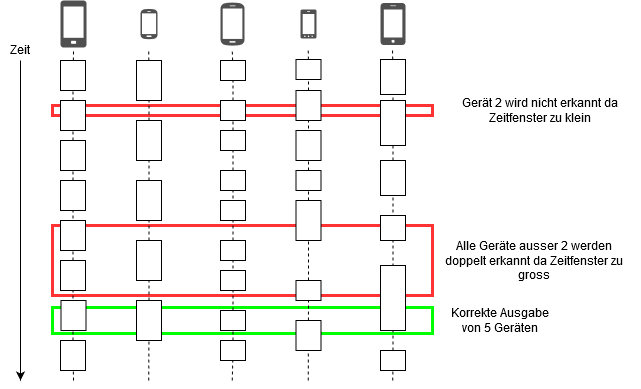
\includegraphics[width=1\linewidth]{Experiments/Zeitfenstermessung.png}
    \caption{Zeitbasierte Filterung von ausgesendeten Probe-Requests
    \label{figure:timewindowfiltering}}
\end{figure}

\clearpage 

Die grösste Schwierigkeit ist dabei, dass das Zeitfenster derart gewählt wird,
dass nicht zwei Bursts eines Geräts als zwei separate Geräte fehlinterpretiert 
werden, oder dass ein Gerät nicht erkannt wird, weil innerhalb des Zeitfensters 
gerade keine Probe-Requests gesendet wurden.
Die Genauigkeit der Messung kann verbessert werden, 
indem mehrere Zeitfenster zu verschiedenen Zeitpunkten ausgewertet werden 
und ein Mittelwert aus den Resultaten gebildet wird.
Zudem kann eine Auswertung der Burst-Zwischenankunfts-zeiten zur Laufzeit 
dazu verwendet werden, das Zeitfenster dynamisch an die Umgebung anzupassen

\paragraph{Umsetzbarkeit}
Dieser Ansatz lässt sich mit wenig Aufwand umsetzen, vorausgesetzt, die 
Probe-Requests werden bereits durch eine Vorfilterung in Bursts aufgeteilt.
Weiterhin ist dieser Ansatz gegenüber einer Veränderung von Geräteverhalten 
robust, da nur die Zwischenankunftszeiten der Bursts für die Unterteilung
benötigt werden.
Allerdings ist die Genauigkeit dieser Filterregel eher gering, da die 
Unterteilung in erster Linie von der Wahl der Dauer des Zeitfensters abhängt. 
Die Messergebnisse zeigen, dass ein Zeitbasierter Ansatz umsetzbar ist, 
da aber die verschiedenen getesteten Geräte keine einheitlichen 
Burstgrössen und -Zwischenankunftszeiten haben, muss die optimale Grösse des 
Zeitfensters experimentell ermittelt werden.

\subsubsection*{Ansatz 2 - Auswertung der Information Element Felder}
Dieser Ansatz beinhaltet zwei Vorgehen:
Zum einen kann aufgrund vorhandener IE-Felder ein Mobilgerät von einem 
anderen unterschieden werden, wenn sie nicht dieselben Felder in ihren 
Probe-Requests verwenden.
Zum anderen können Parameter in diesen Feldern dazu verwendet werden,
Geräte zu unterscheiden.

Der Ansatz wurde auch schon in verwandten Arbeiten angewendet und die 
Messergebnisse lassen darauf schliessen, dass er auch weiterhin für 
ein Fingerprinting verwendet werden kann.

\paragraph{Vorgehen}
Eintreffende Probe-Request werden nach ihren IE-Feldern sortiert und in 
distinkte Gruppen unterteilt. 
Im Idealfall befindet sich pro Gruppe nur ein einzelnes Mobilgerät.
Da gemäss unseren Messergebnissen aber mehrere Geräte die selben IE-Felder 
in ihren Probe-Requests verwenden und die Parameter in diesen Feldern 
auch identisch sein können, werden aber in jeder Gruppe mehrere Geräte auftreten.
Ein weiteres Problem ist die Tatsache, dass ein Mobilgerät in mehreren Bursts
nicht die selben IE-Felder verwenden muss. 
Somit ist es möglich, dass Bursts eines Geräts als mehrere Mobilgeräte erkannt 
werden.

\paragraph{Umsetzbarkeit}
Das Auslesen und Auswerten von Information Element Feldern aus Probe-Requests 
kann mit geringem Aufwand durchgeführt werden.

\subsubsection*{Ansatz 3 - Filtern von nichtrandomisierten MAC-Adressen}
Wird die gleiche MAC-Adresse über mehrere Bursts erkannt, kann davon ausgegangen 
werden, dass das Gerät die MAC-Adresse nicht randomisiert. In diesem Fall kann
eine Filterung gemäss der Abbildung~\ref{figure:naivefingerprinting} durchgeführt
und die MAC-Adresse des Geräts als Fingerabdruck verwendet werden.

\paragraph{Vorgehen}
Parallel zu anderen Filtern kann die wiederholte Verwendung von MAC-Adressen über
mehrere Bursts erkannt werden. Weitere Bursts mit dieser Adresse können direkt 
mit dem Fingerabdruck versehen werden.

\paragraph{Umsetzbarkeit}
Wenn bereits eine Gruppierung von Probe-Requests nach Bursts vorgenommen wurde,
benötigt die Umsetzung dieses Verfahrens nur geringen Aufwand.

\subsubsection*{Ansatz 4 - Filterung zur Laufzeit anhand Burst-Zwischenanktunftszeiten}
Wenn für sämtliche Gerätetypen und Betriebssysteme die Zwischenankunftszeiten
bekannt ist, und diese sich deterministisch verhalten, ist es möglich, 
eintreffende Bursts anhand dieser Zeiten einem bekannten gerät zuzuordnen.

\paragraph{Vorgehen}
Angenommen, man hat ein Mobilgerät, welches immer 30 Sekunden nach dem 
letzten Probe-Request einen neuen Burst aussendet. 
Somit spielt es keine Rolle, ob die MAC-Adresse in jedem Burst neu 
zufallsgeneriert wird, da man nach einer Messung nur die 30s wartet und 
den neuen Burst für den Fingerprint aktualisiert.

Dieses Vorgehen hat mehrere Schwächen:
\begin{itemize}
    \item Falls ein Mobilgerät die Bursts nicht immer in gleichbleibenden 
    Abständen aussendet, lässt sich das Verfahren nicht anwenden.
    \item Wenn zwei Mobilgeräte dieselbe Zwischenankunftszeit haben, 
    können diese nicht unterschieden werden.
    \item Wenn ein Mobilgerät eine Verzögerung von 30s und ein weiteres 
    Mobilgerät eine Verzögerung von 15s haben, 
    kann man diese Geräte alle 30 Sekunden nicht unterscheiden.
    \item Wenn zwei Probe-Requests von unterschiedlichen Mobilgeräten 
    zur gleichen Zeit aufgezeichnet werden, 
    lassen sich die Mobilgeräte nicht unterscheiden

\end{itemize}

\paragraph{Umsetzbarkeit}
In den Versuchen hat sich herausgestellt, dass die meisten Geräte die 
Bursts in zufälligen Zeitintervallen aussenden. 
Somit lässt sich dieses Verfahren nicht generell umsetzen.
In Kombination mit anderen Verfahren kann dieser Ansatz aber dazu verwendet 
werden die Genauigkeit dieser Verfahren zu erhöhen. 
Dazu muss zur Laufzeit ausgewertet werden, ob die Zwischenanktunftszeiten 
von Bursts eines Gerätes deterministisch sind, bevor künftige Probe-Requests 
danach sortiert werden.

\subsubsection*{Ansatz 5 - Bitweise MAC-Header-Analyse}
Im Paper "Noncooperative 802.11 MAC Layer Fingerprinting and Tracking 
of Mobile Devices” aus dem Jahr 2017 wird ein Verfahren beschrieben, 
mit dem ein Fingerprinting und Tracking bewerkstelligt werden könnte.

\paragraph{Verfahren}
Prinzipiell wird jedes Bit des Probe-Request MAC-Headers mittels der 
Berechnung der Entropie über sämtlichen vergangenen Messungen gewichtet. 
Neu auftretende Felder oder selten verwendete Felder haben eine hohe Gewichtung 
und werden für ein Fingerprinting direkt verwendet. 
Felder, die in einer Vielzahl von Probe-Requests vorkommen, 
werden für den Fingerprint ignoriert.

\paragraph{Umsetzbarkeit}
Im Vergleich mit den bisher genannten Verfahren ist dieser Ansatz der 
Aufwändigste und wird voraussichtlich im Rahmen dieser Arbeit nicht umgesetzt.

\subsubsection*{Ansatz 6 - Filterung nach Sequenznummer}
Für Geräte, deren Sequenznummer nicht pro Burst zufallsgeneriert wird,
können Bursts daran erkannt werden, dass die Sequenznummer in neueren 
Frames inkrementiert wird.

\paragraph{Verfahren}
Wird erkannt, dass ein Mobilgerät in mehreren aufeinanderfolgenden 
Bursts die Sequenznummer nicht zufallsgeneriert, 
kann diese Erkenntnis dafür genutzt werden, 
eine Unterscheidung von Mobilgeräten genauer zu machen.
Wenn Beispielsweise mit einem anderen Verfahren die Unterscheidung 
von zwei Bursts nicht möglich ist, aber erkannt wurde, 
dass Gerät A die Sequenznummer nicht randomisiert 
(unabhängig ob B ebenfalls die Sequenznummer nicht randomisiert), 
kann man denjenigen Burst auswählen, dessen Sequenznummer näher an der des 
vorhergehenden Bursts ist.

\paragraph{Umsetzbarkeit}
Die Versuche haben gezeigt, dass mehrere Geräte die Sequenznummern nicht 
für neue Bursts zufallsgenerieren.
In Kombination mit anderen Verfahren bietet diese Lösung eine 
Möglichkeit die Genauigkeit einer Unterscheidung zu erhöhen.

\subsubsection*{Ansatz 7 - Filterung nach Framelänge}
Wenn ein Gerät bei den Probe-Requests immer die gleiche Frame Länge hat, 
können die Probe-Requests dieses Gerätes daran erkannt und von Probes von 
anderen Geräten unterschieden werden.

\paragraph{Verfahren}
Dieses Verfahren ist vom Prinzip her ähnlich wie die Erkennung der IE Felder. 
Es ist allerdings einfacher, ein Frame anhand der Länge, 
die in Wireshark spezifisch ausgegeben wird, zu kategorisieren.

\paragraph{Umsetzbarkeit}
In den Messungen wurde erkannt, dass die Frame-Länge je nach dem messenden 
Gerät unterschiedlich sein kann, 
da abhängig von der Netzwerkkarte unterschiedliche Radiotap Header-Informationen 
aufgezeichnet werden. 
Deshalb wird dieses Verfahren nicht umgesetzt und stattdessen die Filterung nach 
IE-Feldern implementiert.

\subsubsection*{Ansatz 8 - Filtern nach Local-Bit}
Wenn ein Mobilgerät für sämtliche Frames in der zufallsgenerieren MAC-Adresse
das Local-Bit immer setzt, kann dieses Gerät von einem anderen Gerät, 
welches das Local-Bit auch zufällig setzt, unterschieden werden.

\paragraph{Verfahren}
Ähnlich wie in den Verfahren 3 und 6 kann zur Laufzeit evaluiert werden,
ob in einer Gerätegruppe in den Frames der Bursts das Local Bit immer 
gesetzt ist. Künftig aufgezeichnete Frames können danach herausgefiltert werden.

\paragraph{Umsetzbarkeit}
Auch dieses Verfahren kann in Kobmbination mit anderen Verfahren dazu beitragen,
die Genauigkeit einer Unterscheidung zu verbes-sern.

\clearpage